\documentclass[14pt]{extbook}
\usepackage{multicol, enumerate, enumitem, hyperref, color, soul, setspace, parskip, fancyhdr} %General Packages
\usepackage{amssymb, amsthm, amsmath, latexsym, units, mathtools} %Math Packages
\everymath{\displaystyle} %All math in Display Style
% Packages with additional options
\usepackage[headsep=0.5cm,headheight=12pt, left=1 in,right= 1 in,top= 1 in,bottom= 1 in]{geometry}
\usepackage[usenames,dvipsnames]{xcolor}
\usepackage{dashrule}  % Package to use the command below to create lines between items
\newcommand{\litem}[1]{\item#1\hspace*{-1cm}\rule{\textwidth}{0.4pt}}
\pagestyle{fancy}
\lhead{Progress Quiz 10}
\chead{}
\rhead{Version A}
\lfoot{5170-5105}
\cfoot{}
\rfoot{Summer C 2021}
\begin{document}

\begin{enumerate}
\litem{
Choose the equation of the function graphed below.
\begin{center}
    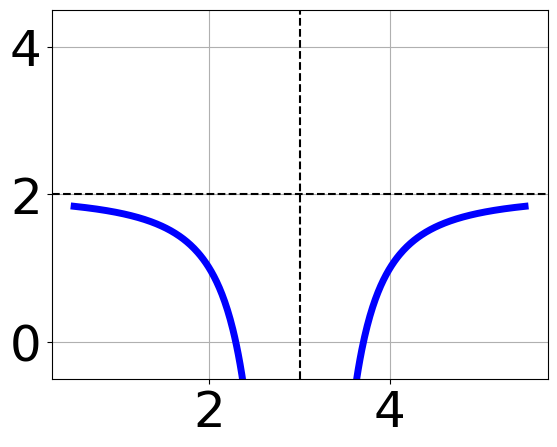
\includegraphics[width=0.5\textwidth]{../Figures/rationalGraphToEquationCopyA.png}
\end{center}
\begin{enumerate}[label=\Alph*.]
\item \( f(x) = \frac{1}{x + 3} + 2 \)
\item \( f(x) = \frac{-1}{(x - 3)^2} + 2 \)
\item \( f(x) = \frac{-1}{x - 3} + 2 \)
\item \( f(x) = \frac{1}{(x + 3)^2} + 2 \)
\item \( \text{None of the above} \)

\end{enumerate} }
\litem{
Solve the rational equation below. Then, choose the interval(s) that the solution(s) belongs to.\[ \frac{-88}{99x + 22} + 1 = \frac{-88}{99x + 22} \]\begin{enumerate}[label=\Alph*.]
\item \( x_1 \in [-1.1, -0.1] \text{ and } x_2 \in [-0.34,-0.04] \)
\item \( x_1 \in [-1.1, -0.1] \text{ and } x_2 \in [0.17,0.28] \)
\item \( x \in [0.1,1.8] \)
\item \( x \in [-0.22,2.78] \)
\item \( \text{All solutions lead to invalid or complex values in the equation.} \)

\end{enumerate} }
\litem{
Determine the domain of the function below.\[ f(x) = \frac{6}{12x^{2} -12} \]\begin{enumerate}[label=\Alph*.]
\item \( \text{All Real numbers.} \)
\item \( \text{All Real numbers except } x = a, \text{ where } a \in [-17.4, -14.6] \)
\item \( \text{All Real numbers except } x = a \text{ and } x = b, \text{ where } a \in [-17.4, -14.6] \text{ and } b \in [8.4, 9.8] \)
\item \( \text{All Real numbers except } x = a, \text{ where } a \in [-3.6, -0.6] \)
\item \( \text{All Real numbers except } x = a \text{ and } x = b, \text{ where } a \in [-3.6, -0.6] \text{ and } b \in [0.1, 2.5] \)

\end{enumerate} }
\litem{
Choose the graph of the equation below.\[ f(x) = \frac{1}{(x - 1)^2} - 2 \]\begin{enumerate}[label=\Alph*.]
\begin{multicols}{2}\item 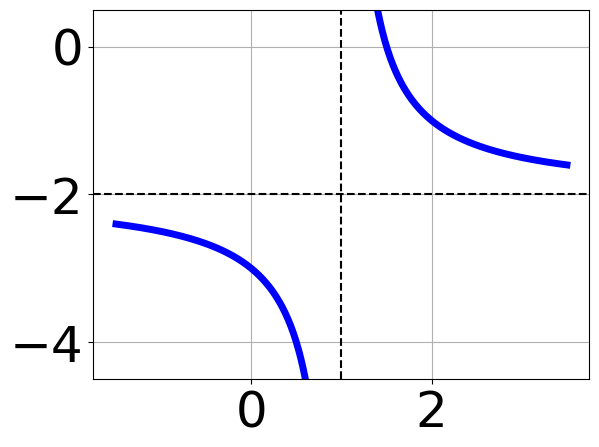
\includegraphics[width = 0.3\textwidth]{../Figures/rationalEquationToGraphCopyAA.png}\item 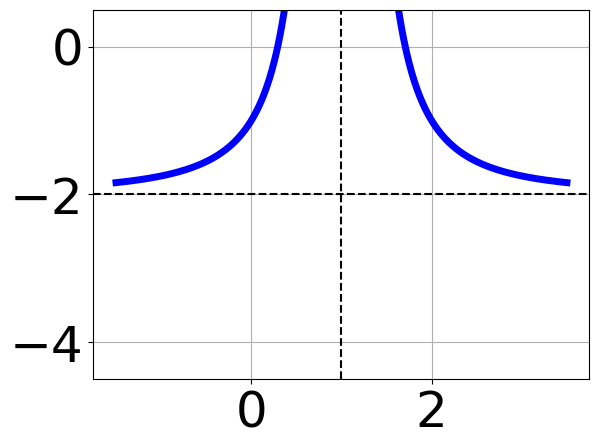
\includegraphics[width = 0.3\textwidth]{../Figures/rationalEquationToGraphCopyBA.png}\item 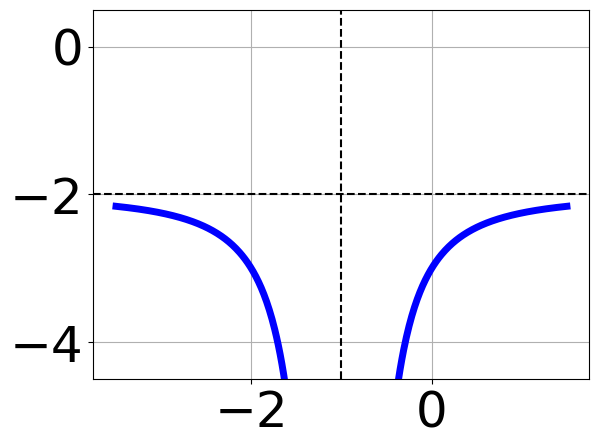
\includegraphics[width = 0.3\textwidth]{../Figures/rationalEquationToGraphCopyCA.png}\item 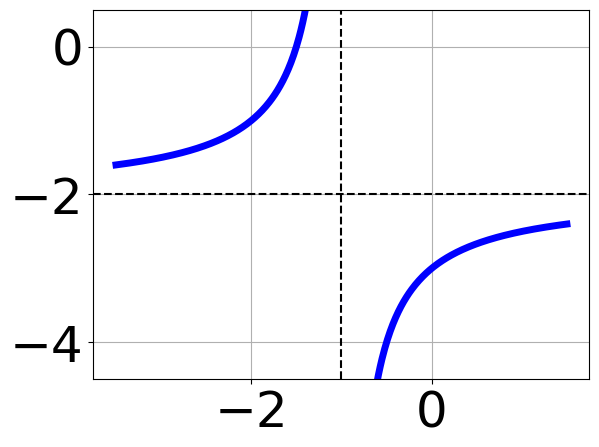
\includegraphics[width = 0.3\textwidth]{../Figures/rationalEquationToGraphCopyDA.png}\end{multicols}\item None of the above.
\end{enumerate} }
\litem{
Solve the rational equation below. Then, choose the interval(s) that the solution(s) belongs to.\[ \frac{4x}{-2x + 3} + \frac{-4x^{2}}{-8x^{2} +4 x + 12} = \frac{7}{4x + 4} \]\begin{enumerate}[label=\Alph*.]
\item \( x \in [-1.33,0.28] \)
\item \( x_1 \in [-0.84, 2.52] \text{ and } x_2 \in [-0.5,4.5] \)
\item \( x_1 \in [-0.84, 2.52] \text{ and } x_2 \in [-11.07,0.93] \)
\item \( \text{All solutions lead to invalid or complex values in the equation.} \)
\item \( x \in [-3.83,-2.24] \)

\end{enumerate} }
\litem{
Choose the equation of the function graphed below.
\begin{center}
    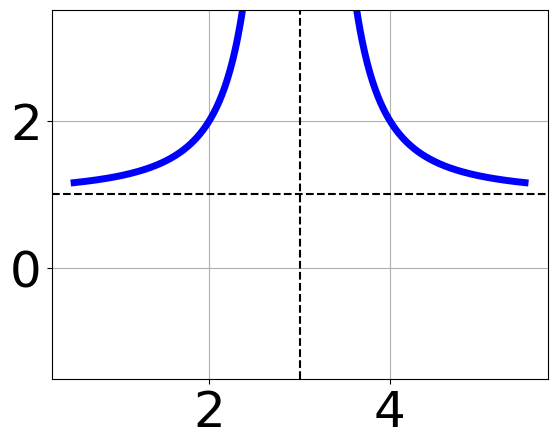
\includegraphics[width=0.5\textwidth]{../Figures/rationalGraphToEquationA.png}
\end{center}
\begin{enumerate}[label=\Alph*.]
\item \( f(x) = \frac{-1}{x - 3} + 8 \)
\item \( f(x) = \frac{-1}{(x - 3)^2} + 8 \)
\item \( f(x) = \frac{1}{(x + 3)^2} + 8 \)
\item \( f(x) = \frac{1}{x + 3} + 8 \)
\item \( \text{None of the above} \)

\end{enumerate} }
\litem{
Determine the domain of the function below.\[ f(x) = \frac{6}{9x^{2} -27 x + 18} \]\begin{enumerate}[label=\Alph*.]
\item \( \text{All Real numbers.} \)
\item \( \text{All Real numbers except } x = a, \text{ where } a \in [8.93, 9.88] \)
\item \( \text{All Real numbers except } x = a \text{ and } x = b, \text{ where } a \in [0.73, 1.14] \text{ and } b \in [1.29, 2.13] \)
\item \( \text{All Real numbers except } x = a, \text{ where } a \in [0.73, 1.14] \)
\item \( \text{All Real numbers except } x = a \text{ and } x = b, \text{ where } a \in [8.93, 9.88] \text{ and } b \in [17.21, 18.34] \)

\end{enumerate} }
\litem{
Choose the graph of the equation below.\[ f(x) = \frac{-1}{x - 3} - 2 \]\begin{enumerate}[label=\Alph*.]
\begin{multicols}{2}\item 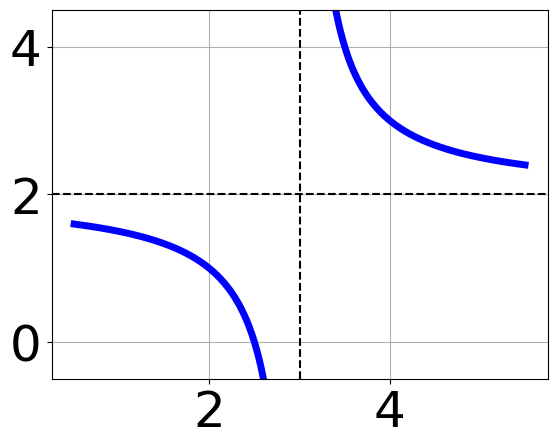
\includegraphics[width = 0.3\textwidth]{../Figures/rationalEquationToGraphAA.png}\item 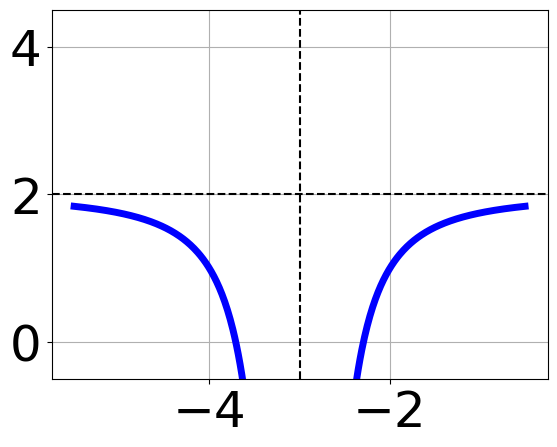
\includegraphics[width = 0.3\textwidth]{../Figures/rationalEquationToGraphBA.png}\item 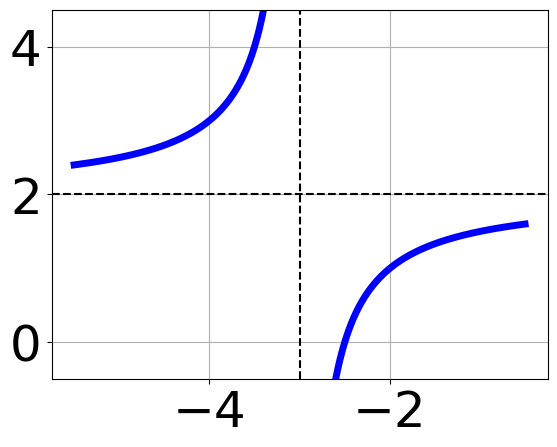
\includegraphics[width = 0.3\textwidth]{../Figures/rationalEquationToGraphCA.png}\item 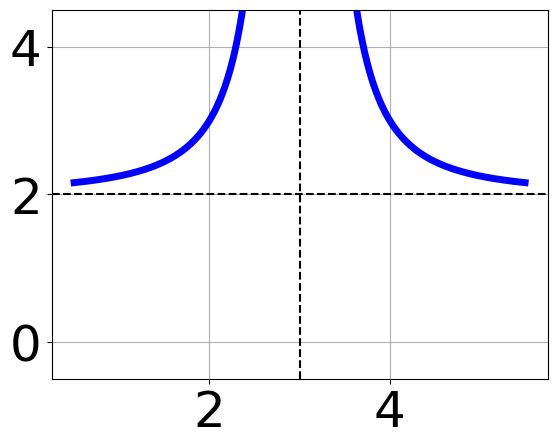
\includegraphics[width = 0.3\textwidth]{../Figures/rationalEquationToGraphDA.png}\end{multicols}\item None of the above.
\end{enumerate} }
\litem{
Solve the rational equation below. Then, choose the interval(s) that the solution(s) belongs to.\[ \frac{7x}{6x + 6} + \frac{-4x^{2}}{36x^{2} +60 x + 24} = \frac{-7}{6x + 4} \]\begin{enumerate}[label=\Alph*.]
\item \( x_1 \in [-1.14, -0.86] \text{ and } x_2 \in [-0.7,-0.47] \)
\item \( \text{All solutions lead to invalid or complex values in the equation.} \)
\item \( x_1 \in [-1.47, -1.1] \text{ and } x_2 \in [-0.59,-0.06] \)
\item \( x \in [-1.14,-0.86] \)
\item \( x \in [-0.76,-0.61] \)

\end{enumerate} }
\litem{
Solve the rational equation below. Then, choose the interval(s) that the solution(s) belongs to.\[ \frac{20}{-40x + 20} + 1 = \frac{20}{-40x + 20} \]\begin{enumerate}[label=\Alph*.]
\item \( x \in [0.5,2.5] \)
\item \( x_1 \in [-1, 0.1] \text{ and } x_2 \in [-0.5,2.5] \)
\item \( x \in [-1,0.1] \)
\item \( x_1 \in [0, 1.1] \text{ and } x_2 \in [-0.5,2.5] \)
\item \( \text{All solutions lead to invalid or complex values in the equation.} \)

\end{enumerate} }
\end{enumerate}

\end{document}